% begin module curve-sketching-ex6
\begin{frame}
\begin{example}[Example 4, p. 275]
Discuss the curve $y = \alert<handout:0| 19-20,39-42>{f(x)}$ \alert<handout:0| 19-20,39-42>{$= x^4 - 4x^3$} with respect to \alert<handout:0| 28-35>{concavity}, \alert<handout:0| 36-42>{points of inflection}, and \alert<handout:0| 10-27>{local maxima and minima}.  \alert<handout:0| 43->{Sketch the curve.}
\begin{columns}[c]
\column{.42\textwidth}
\ \only<handout:0| -19>{%
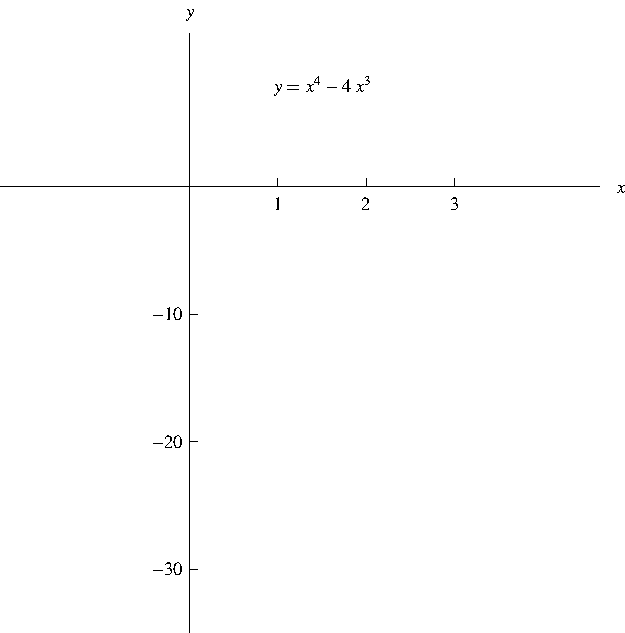
\includegraphics[height=4.5cm]{curve-sketching/pictures/04-03-ex6a.pdf}%
}%
\only<handout:0| 20-39>{%
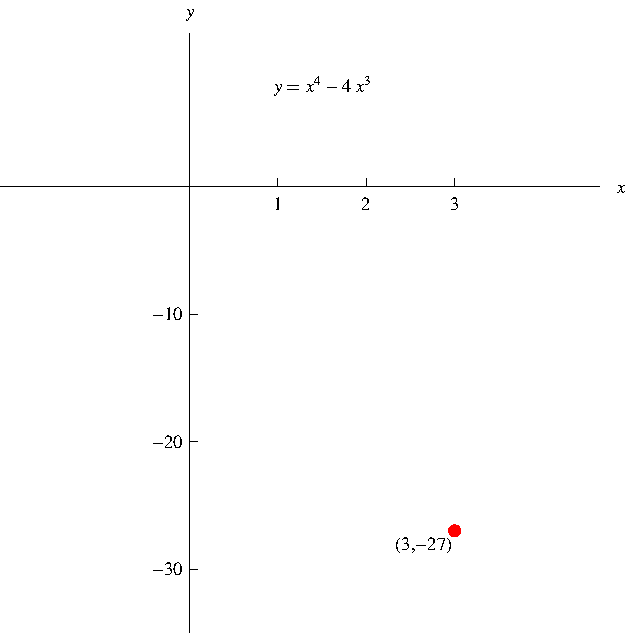
\includegraphics[height=4.5cm]{curve-sketching/pictures/04-03-ex6b.pdf}%
}%
\only<handout:0| 40-41>{%
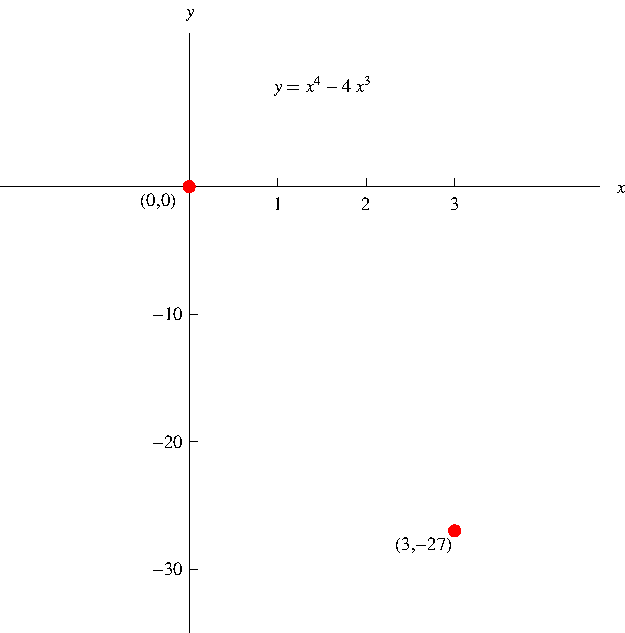
\includegraphics[height=4.5cm]{curve-sketching/pictures/04-03-ex6c.pdf}%
}%
\only<handout:0| 42-43>{%
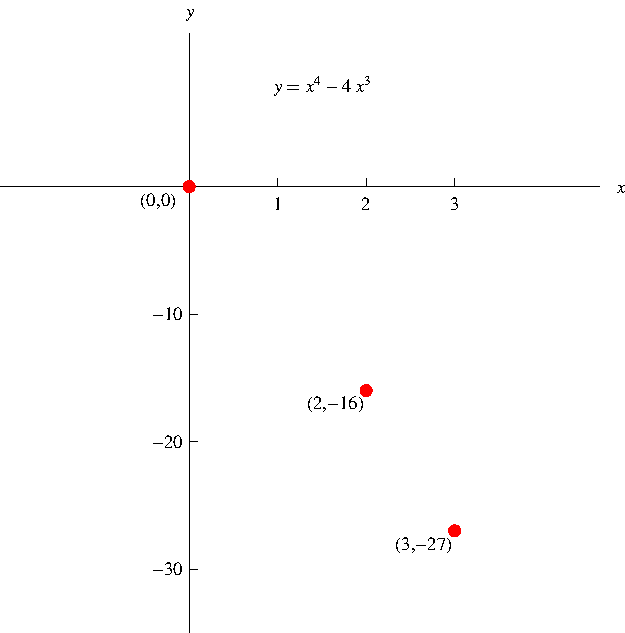
\includegraphics[height=4.5cm]{curve-sketching/pictures/04-03-ex6d.pdf}%
}%
\only<handout:0| 44-45>{%
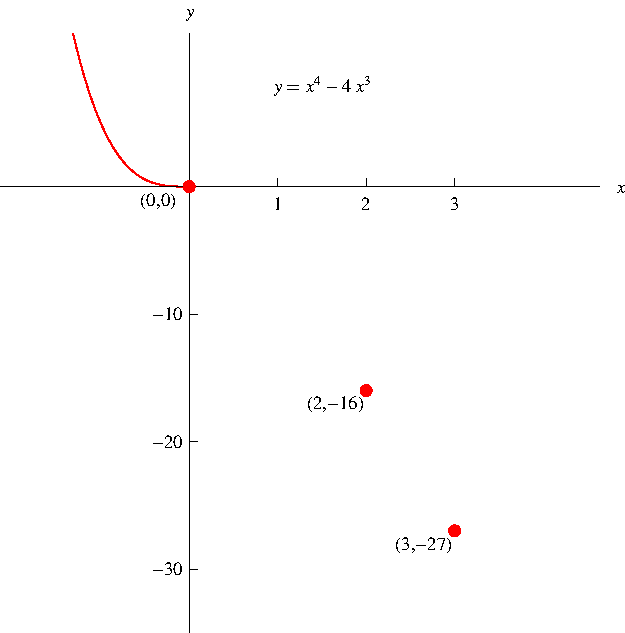
\includegraphics[height=4.5cm]{curve-sketching/pictures/04-03-ex6e.pdf}%
}%
\only<handout:0| 46-47>{%
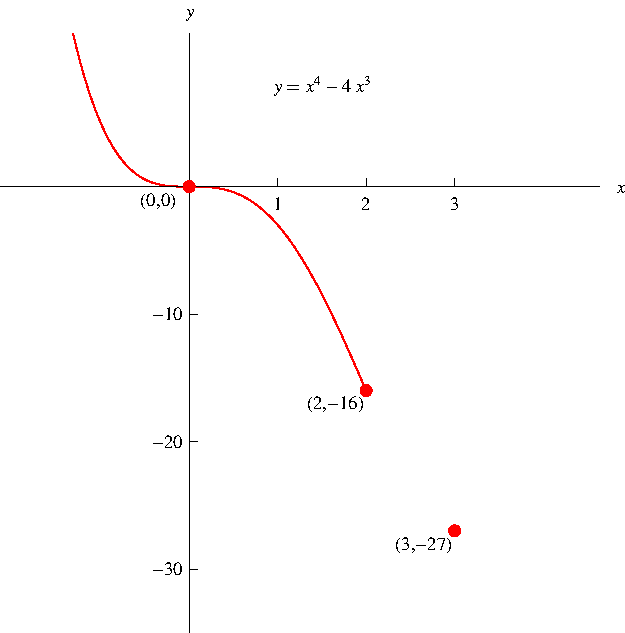
\includegraphics[height=4.5cm]{curve-sketching/pictures/04-03-ex6f.pdf}%
}%
\only<48->{%
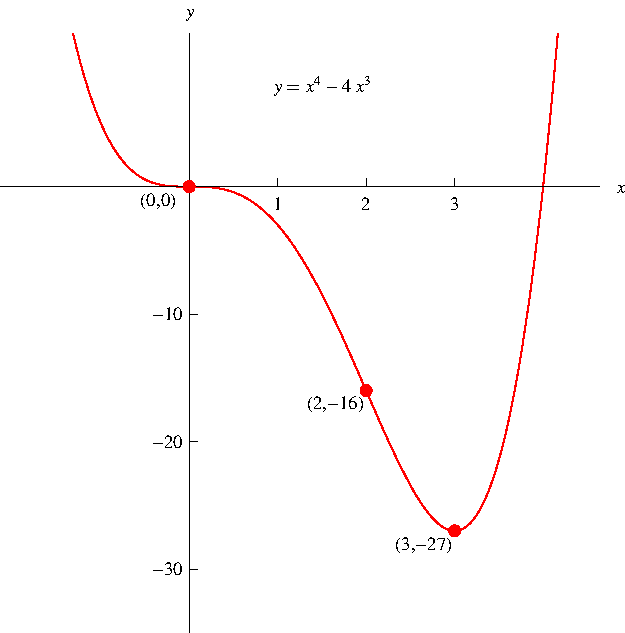
\includegraphics[height=4.5cm]{curve-sketching/pictures/04-03-ex6g.pdf}%
}%
\vspace{.1in}

\uncover<28->{%
\ \ \ \begin{tabular}{|@{\ }r@{\ }|@{\ }c@{\ }|@{\ }l@{\ }|}
\hline
Interval & $f''(x)$ & \alert<handout:0| 35,43-48>{Concave}\\
\hline
\alert<handout:0| 29-30,37,43-44>{$(-\infty , 0)$} &%
\uncover<30->{\alert<handout:0| 30,37>{$+$}} &%
\uncover<35->{\alert<handout:0| 35,43-44>{up}}\\
\alert<handout:0| 31-32,37-38,45-46>{$(0, 2)$} &%
\uncover<32->{\alert<handout:0| 32,37-38>{$-$}} &%
\uncover<35->{\alert<handout:0| 35,45-46>{down}}\\
\alert<handout:0| 33-34,38,47-48>{$(2, \infty )$} &%
\uncover<34->{\alert<handout:0| 34,38>{$+$}} &%
\uncover<35->{\alert<handout:0| 35,47-48>{up}}\\
\hline
\end{tabular}
}%
\column{.58\textwidth}
\begin{itemize}
\item<2-| alert@2-3,23-26>  $f'(x) = $ \alert<handout:0| 4-5>{\uncover<3->{$4x^3 - 12x^2$} \uncover<4->{$ = $}\uncover<5->{$4\alert<handout:0| 11>{x^2}\alert<handout:0| 12>{(x-3)}$.}}
\item<2-| alert@6-7,29-34>  \alert<handout:0| 13-16>{$f''(x) = $} \alert<handout:0| 8-9>{\uncover<7->{\alert<handout:0| 13-16>{$12x^2 - 24x$}} \uncover<8->{$ = $} \uncover<9->{$12x(x-2)$.}}
\item<10->  Critical numbers: \uncover<11->{\alert<handout:0| 11,21-22>{$0$}} and \uncover<12->{\alert<handout:0| 12,17-18>{$3$}.}
\item<13->  \alert<handout:0| 13-14,21-22>{$f''(0) = \uncover<14->{0}$} and \alert<handout:0| 15-18>{$f''(3) =$ \uncover<16->{$36 > 0$.}}
\item<17->  Second Derivative Test:
\item<17-| alert@17-18>  \alert<handout:0| 47-48>{Local \uncover<18->{minimum} at $3$.}  \alert<handout:0| 19-20>{\uncover<19->{$f(3) =$ \uncover<20->{$-27$.}}}
\item<22-| alert@22>  No information about $0$.
\item<23->  First Derivative Test:
\item<23->  \alert<handout:0| 23-24>{$f'$ is \uncover<24->{$-$} on $(-\infty , 0)$} \alert<handout:0| 25-26>{and \uncover<26->{$-$} on $(0, 3)$}.
\item<27->  No local max or min at $0$.
\item<36->  Inflection points: \alert<handout:0| 39-40>{$\uncover<39->{(}\uncover<37->{\alert<handout:0| 37>{0}}\uncover<39->{,\uncover<40->{0})}$} and \alert<handout:0| 41-42>{$\uncover<39->{(}\uncover<38->{\alert<handout:0| 38>{2}}\uncover<39->{,\uncover<42->{-16})}$}
\end{itemize}
\end{columns}
\end{example}
\end{frame}
% end module curve-sketching-ex6
